\chapter{第4章 移动端STANDING信号处理算法设计}

\section{引言}

随着移动设备计算能力的提升和内置传感器精度的不断改进,利用智能手机等移动端设备进行前庭功能评估成为可能。与传统专业设备相比,移动端前庭评估具有便携性强、成本低廉、操作简便等显著优势,特别适用于基层医疗机构和资源有限地区。然而,移动端设备采集的前庭信号存在采样率较低、信噪比不佳、运动伪影多等缺点,给信号处理和特征提取带来挑战。本章将重点讨论移动端STANDING信号处理算法设计,包括前庭信号预处理、头脉冲试验(HIT)参数计算以及眼震模式识别等关键环节,旨在解决移动平台信号质量受限条件下的精确前庭功能评估问题。

\section{移动端前庭信号采集与特点}

\subsection{信号采集原理}

移动端前庭信号主要通过内置摄像头采集眼动视频,同时利用陀螺仪和加速度计记录头部运动数据。眼动信号的获取基于瞳孔追踪算法,通过视频图像处理技术实时检测瞳孔位置变化,从而提取水平和垂直方向的眼球运动轨迹。头部运动数据则依靠移动设备内置的惯性传感器直接记录角速度和加速度信息。

与专业设备的硬件限制对比,移动端前庭信号具有以下特点:

\begin{enumerate}
  \item \textbf{采样率受限}:专业设备通常可达250Hz以上采样率,而移动设备受限于摄像头帧率,眼动数据采样率一般仅为30-60Hz,无法完整捕捉高频眼动成分。

  \item \textbf{噪声干扰显著}:由于光线条件不稳定、手持晃动以及计算资源限制,移动设备采集的信号常伴随高频噪声和基线漂移。

  \item \textbf{信号不连续性}:瞳孔跟踪过程中的眨眼、遮挡等因素导致信号中存在间断点和异常值,需要特殊处理策略。

  \item \textbf{时间同步问题}:眼动数据与头动数据来自不同传感器,存在微秒级延迟,需要精确时间同步以确保计算准确性。

  \item \textbf{设备差异性}:不同移动设备的摄像头性能、传感器精度存在差异,算法需具备适应性以应对各类设备平台。
\end{enumerate}

这些特点决定了移动端前庭信号处理算法必须具备强大的抗干扰能力和适应性,才能从质量有限的原始数据中提取可靠的诊断特征。

\section{前庭信号预处理算法}

\subsection{信号预处理架构}

针对移动端采集的前庭信号特点,我们设计了一套系统化的预处理流程,以提高信号质量并为后续特征提取提供可靠基础。整体预处理架构如图\ref{fig:signal_preprocess}所示。

\begin{figure}[ht]
    \centering
    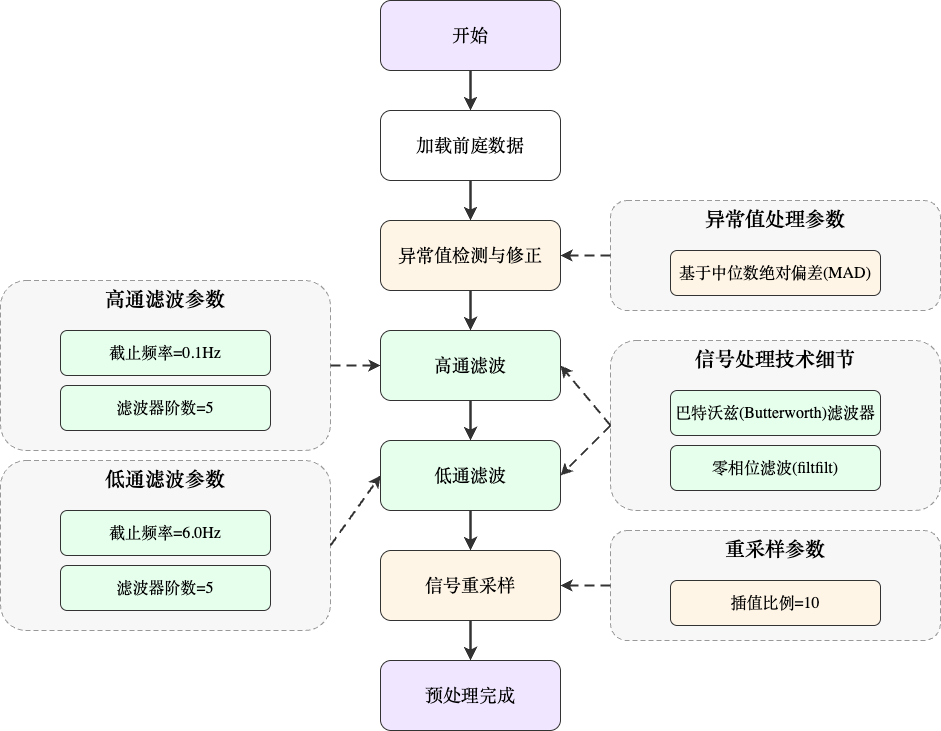
\includegraphics[width=0.85\textwidth]{chapter_4/signal_preprocess.png}
    \caption{信号预处理架构图}
    \label{fig:signal_preprocess}
\end{figure}

预处理流程主要包括以下几个核心步骤:数据加载与标准化、基线漂移校正、异常值检测与处理、多级滤波以及信号重采样,各环节紧密配合以实现从原始数据到高质量分析信号的转换。

\subsection{多级滤波算法}

移动端采集的前庭信号常伴随多种频率成分的噪声,我们采用多级滤波策略有效分离有用信号与噪声。

\subsubsection{高通滤波去除基线漂移}

眼动和头动信号中的低频基线漂移主要源于设备移动、姿势变化等因素,高通滤波器能有效去除这类干扰。我们采用巴特沃兹(Butterworth)高通滤波器,其数学表达式为:

\begin{equation}
H(s) = \frac{s^n}{s^n + \omega_c^n}
\end{equation}

其中,$n$为滤波器阶数,$\omega_c$为截止频率。在实际处理中,截止频率设定为0.1Hz,阶数为5。与传统FIR滤波器相比,巴特沃兹滤波器在通带内具有最大平坦特性,可以更好地保留眼震和头脉冲信号的完整性。

滤波过程采用零相位滤波技术实现,可有效避免相位失真导致的时序特征偏移,这对于眼震模式的准确检测至关重要。

\subsubsection{低通滤波消除高频噪声}

移动设备采集的信号常含有高频噪声,包括传感器噪声、瞳孔检测抖动等。我们设计了阈值为6Hz的低通滤波器,根据眼震和头脉冲信号的频率特性,此设置能够有效保留主要生理信号成分的同时最大程度抑制高频噪声。低通滤波同样采用巴特沃兹设计,阶数设为5以获得较陡峭的过渡带和良好的阻带衰减性能。

通过滤波参数的精确调节,我们可以在移动端设备的计算资源限制下实现对信号的高效滤波。

\subsection{信号重采样与插值}

移动设备采集的眼动信号采样率通常不足,难以捕捉高速眼动的完整轮廓。为解决此问题,我们设计了基于三次样条插值的信号重采样算法,其核心思想是在保持信号原有形态的前提下,提高采样点密度,改善峰值检测和斜率计算的精度。

重采样过程可表示为:

\begin{equation}
x_{new}(t_i) = S(t_i), \quad t_i = t_0 + i \cdot \frac{t_n - t_0}{n \cdot r}
\end{equation}

其中,$S(t)$为三次样条插值函数,$r$为插值比例(通常设为10),$n$为原始采样点数量。与简单的线性插值相比,三次样条插值能更好地保留眼动信号的曲率特性,减少过冲和振铃现象,特别适合眼震信号中快相与慢相的精确刻画。

在实际应用中,重采样步骤大幅提高了后续拐点检测的准确性和稳定性,对于低质量原始信号的特征提取尤为关键。

\subsection{异常值检测与修正}

移动设备采集的前庭信号常含有由眨眼、视线偏移等引起的异常值,如果不加处理,将严重影响特征提取的准确性。我们采用基于滑动中位数绝对偏差(MAD)的异常值检测方法,具体定义为:

\begin{equation}
\text{MAD} = \text{median}(|x_i - \text{median}(x)|)
\end{equation}

\begin{equation}
\text{threshold} = \text{median}(x) \pm \alpha \cdot \text{MAD}
\end{equation}

其中,$\alpha$为调节参数,通常设为3.5。相比传统基于均值和标准差的方法,MAD对极端异常值更加鲁棒,适合前庭信号中可能出现的突发异常。

对于检测到的异常值,我们采用局部三次样条插值进行修正,而非简单剔除,以确保信号连续性和特征完整性。这种方法在保持前庭信号主要特征的同时,有效降低了异常值对后续分析的干扰。

\subsection{预处理综合策略}

以上预处理步骤并非独立应用,而是作为一个有机整体协同工作。具体流程如下:

\begin{enumerate}
  \item 首先对原始信号进行异常值检测与修正,去除明显错误点
  \item 应用高通滤波去除基线漂移,确保信号在合理基准线上波动
  \item 再通过低通滤波消除高频噪声,提取主要生理信号成分
  \item 最后进行信号重采样,提高采样密度以便更精确地捕捉信号特征
\end{enumerate}

这种多步骤级联处理策略能够最大限度地提高移动端采集信号的质量,为后续的特征提取奠定坚实基础。通过系统化的参数调优和算法验证,预处理模块已能够适应不同移动设备和检查环境,展现出良好的泛化能力。

\section{头脉冲试验(HIT)参数计算算法}

头脉冲试验是STANDING法中评估前庭-眼反射功能的关键环节。在移动端实现中,我们需要特别关注如何从有限质量的眼动和头动数据中精确计算VOR增益值。

\subsection{头脉冲事件检测}

准确识别头脉冲事件是计算VOR增益的首要步骤。与传统设备不同,移动端采集的头动数据采样率相对较低,难以依靠简单阈值检测准确捕捉头脉冲起止时间。我们设计了一种改进的多阈值自适应检测算法,结合角速度和角加速度信息,实现头脉冲事件的精确定位。

头脉冲事件检测算法的核心逻辑如下:

\begin{enumerate}
  \item \textbf{预处理}:对头动角速度信号应用低通滤波,去除高频噪声,保留头脉冲主要特征
  \item \textbf{候选区域识别}:设定初始阈值$\omega_{threshold}$(通常为50°/s),标记所有角速度超过阈值的区间
  \item \textbf{角加速度验证}:计算候选区域的角加速度最大值,必须超过预设阈值$\alpha_{threshold}$(通常为1000°/s²)
  \item \textbf{持续时间约束}:头脉冲事件持续时间应符合生理学特性,通常在100-200ms范围内
  \item \textbf{方向判断}:根据角速度主导方向确定头脉冲为左侧或右侧
\end{enumerate}

该算法的优势在于综合考虑了角速度、角加速度和时间特性,有效避免了单一阈值导致的误检和漏检问题,并能适应不同检查者施加的头脉冲强度差异。

\subsection{眼动-头动同步校准}

移动设备中眼动和头动数据来自不同传感器,存在采样率不一致和时间延迟问题。为确保VOR增益计算准确性,我们设计了基于互相关的信号同步算法。其数学表达式为:

\begin{equation}
R_{eh}(\tau) = \sum_{t} e(t) \cdot h(t+\tau)
\end{equation}

其中,$e(t)$为眼动信号,$h(t)$为头动信号,$\tau$为时间延迟量。算法通过寻找使$R_{eh}(\tau)$取最大值的$\tau$,确定两信号之间的最佳对齐位置。

在实际应用中,我们采用分段互相关策略,将整个记录分为多个小段独立计算延迟,并通过加权平均得到最终延迟值,这种方法能更好地适应检查过程中可能出现的延迟动态变化。

\subsection{VOR增益计算}

VOR增益是头脉冲试验最关键的量化指标,定义为眼球运动速度与头部运动速度的比值。在移动端STANDING系统中,我们采用改进的面积法计算VOR增益,其数学表达式为:

\begin{equation}
\text{Gain} = \frac{\int_{t_1}^{t_2} |v_{eye}(t)| dt}{\int_{t_1}^{t_2} |v_{head}(t)| dt}
\end{equation}

其中,$t_1$和$t_2$为头脉冲事件的起始和结束时间,$v_{eye}(t)$和$v_{head}(t)$分别为眼动和头动的角速度。与传统的峰值比值法相比,面积法考虑了整个头脉冲过程的动态响应,对采样率低和信噪比不佳的情况更加鲁棒。

为提高计算精度,我们引入了以下优化策略:

\begin{enumerate}
  \item \textbf{选择性积分窗口}:仅对头脉冲加速阶段(通常为前100ms)进行积分,避免后期代偿性扫视干扰
  \item \textbf{方向一致性约束}:积分前确保眼动和头动方向一致,即$v_{eye}$与$v_{head}$符号相反
  \item \textbf{异常值过滤}:通过中位数绝对偏差法滤除单次增益计算中的异常值
\end{enumerate}

\subsection{增益不对称率计算}

增益不对称率是评估前庭功能左右平衡性的重要指标,在STANDING诊断中具有重要价值。移动端算法中,我们采用如下公式计算增益不对称率:

\begin{equation}
\text{Asymmetry} = \frac{|G_L - G_R|}{G_L + G_R} \times 100\%
\end{equation}

其中,$G_L$和$G_R$分别为左向和右向头脉冲的平均VOR增益。

为提高不对称率计算的可靠性,我们引入了基于四分位距的异常值过滤机制,排除可能存在的不合理增益值后再计算不对称率,从而减少个别误测对最终结果的影响。

\subsection{扫视检测算法}

代偿性扫视是头脉冲试验中的关键诊断特征,尤其是隐蔽性扫视的检出对前庭功能评估至关重要。在移动端系统中,我们设计了特别适合低采样率条件下的扫视检测算法,主要包含以下步骤:

\begin{enumerate}
  \item \textbf{速度信号预处理}:对眼动速度信号应用自适应阈值滤波,突出扫视特征
  \item \textbf{候选扫视识别}:标记眼动速度超过阈值(一般为40°/s)且方向与头动相同的区域
  \item \textbf{形态学验证}:分析候选区域的加速度、持续时间和振幅特征,确认符合扫视特性
  \item \textbf{分类}:根据扫视发生时间相对于头脉冲峰值的位置,将扫视分为显性(overt)和隐蔽性(covert)
\end{enumerate}

移动端扫视检测的难点在于低采样率条件下可能错过扫视峰值,导致漏检。我们通过扩展检测窗口并引入形态学验证步骤,有效提高了检出率,即使在30Hz采样率条件下也能达到可接受的检测性能。

\section{眼震模式识别算法}

眼震检查是STANDING方法中评估中枢性与外周性眩晕的另一关键环节。与传统设备不同,移动端眼震分析面临采样率低、信噪比差等挑战,需要特殊设计的算法提取可靠眼震特征。

\subsection{眼震模式识别整体框架}

移动端眼震模式识别算法的整体架构如图\ref{fig:nystagmus_detection}所示,包含信号预处理、拐点检测、斜率计算、模式识别和特征计算等关键步骤。

\begin{figure}[ht]
    \centering
    \includegraphics[width=0.85\textwidth]{chapter_4/   nystagmus_autodetction_flowchart.png}
    \caption{眼震自动检测流程图}
    \label{fig:nystagmus_detection}
\end{figure}

该算法的创新点在于采用基于拐点的几何形态识别策略,而非传统的速度阈值法,这种方法特别适合移动端低采样率条件下的眼震检测,能够有效捕捉眼震的快相和慢相交替模式。

\subsection{拐点检测算法}

拐点是眼动信号中方向发生变化的关键点,代表了眼震中快相与慢相的转换位置。准确检测这些拐点是眼震模式识别的基础。我们设计的拐点检测算法基于局部极值原理,并引入了突出度(prominence)参数以滤除微小波动,其主要步骤如下:

\begin{enumerate}
  \item \textbf{局部极值搜索}:在滤波后的眼动信号中搜索满足局部最大或最小条件的点
  \item \textbf{突出度计算}:对每个极值点计算其相对于邻近区域的突出高度
  \item \textbf{阈值筛选}:仅保留突出度超过预设阈值(默认0.1°)的极值点
  \item \textbf{距离约束}:设定相邻拐点间的最小距离(默认150ms),避免过密检测
\end{enumerate}

该算法的数学表达如下:
对于时间序列$x[n]$,点$i$为局部极大值需满足:
\begin{equation}
x[i] > x[i-k] \text{ 且 } x[i] > x[i+k] \text{ 对所有 } 1 \leq k \leq w
\end{equation}

其中$w$为局部窗口宽度。

突出度定义为:
\begin{equation}
p[i] = \min(\max_{i-l \leq j < i}(x[i] - x[j]), \max_{i < j \leq i+r}(x[i] - x[j]))
\end{equation}

其中$l$和$r$为向左右搜索的距离。

与传统的一阶或二阶导数检测法相比,基于突出度的拐点检测对噪声和小幅波动更具鲁棒性,特别适合移动端采集的眼动信号。

\subsection{眼震模式识别策略}

眼震的典型特征是快相和慢相的交替出现。在我们的算法中,通过分析相邻拐点之间的时间间隔和斜率特征来识别眼震模式。具体识别过程如下:

\begin{enumerate}
  \item \textbf{斜率计算}:对每对相邻拐点计算斜率,表示眼球运动速度
   \begin{equation}
   \text{slope}_{i} = \frac{x[t_{i+1}] - x[t_i]}{t_{i+1} - t_i}
   \end{equation}

  \item \textbf{模式匹配}:寻找符合以下条件的连续三个拐点(形成快相-慢相或慢相-快相组合):
   \begin{itemize}
     \item 时间约束:相邻拐点间隔在预设范围内(通常0.3-0.8秒)
     \item 斜率比例约束:快相斜率与慢相斜率的绝对比值在预设范围内(通常1.4-8.0)
     \item 方向约束:快相和慢相斜率符号相反
   \end{itemize}

  \item \textbf{优先级排序}:当多个可能的拐点组合重叠时,优先选择斜率比例更符合眼震特征的组合
\end{enumerate}

该算法的关键创新在于不依赖固定速度阈值,而是基于斜率比例进行识别,这使其能够适应不同强度的眼震,包括微小眼震和大幅眼震,提高了算法的普适性。

\subsection{慢相速度(SPV)计算}

慢相速度(SPV)是眼震定量分析的核心指标,在眩晕鉴别诊断中具有重要价值。针对移动端信号特点,我们设计了基于中位数的健壮SPV计算方法,具体步骤如下:

\begin{enumerate}
  \item \textbf{慢相片段提取}:从识别的眼震模式中提取所有慢相片段
  \item \textbf{斜率计算}:对每个慢相片段计算其斜率(即瞬时速度)
  \item \textbf{中位数估计}:采用中位数而非均值计算SPV,避免异常值干扰
   \begin{equation}
   \text{SPV} = \text{median}(\text{slow\_phase\_slopes})
   \end{equation}
  \item \textbf{变异系数计算}:通过中位数绝对偏差(MAD)计算健壮变异系数
   \begin{equation}
   \text{CV} = \frac{\text{MAD} \times 1.4826}{|\text{median}|} \times 100\%
   \end{equation}
\end{enumerate}

中位数方法相比均值法具有更强的抗干扰能力,特别适合移动端可能存在噪声和伪影较多的情况。同时,变异系数提供了眼震稳定性的量化指标,对判断眼震的生理意义具有重要参考价值。

\subsection{眼震方向判断}

眼震方向是鉴别中枢性与外周性眩晕的关键特征之一。在移动端STANDING系统中,我们基于慢相方向确定眼震方向,算法逻辑如下:

\begin{enumerate}
  \item \textbf{慢相极性统计}:统计所有识别出的慢相斜率的符号
  \item \textbf{多数投票}:采用多数投票法确定主导方向
   \begin{equation}
   \text{direction} = \begin{cases}
   \text{left}, & \text{if } \sum_{i} \text{sign}(\text{slope}_i) < 0 \\
   \text{right}, & \text{if } \sum_{i} \text{sign}(\text{slope}_i) > 0
   \end{cases}
   \end{equation}
  \item \textbf{方向映射}:根据检查使用的参考坐标系统,将左右方向适当映射为水平或垂直坐标
\end{enumerate}

需要特别注意的是,眼震方向判断必须结合具体检查情境,特别是视靶方向。例如,在水平方向视靶诱发的眼震中,应使用水平坐标系判断左右方向;而在垂直方向视靶诱发的眼震中,则应使用垂直坐标系判断上下方向。

\subsection{眼震模式过滤与验证}

移动端采集的眼动信号可能导致误检,为提高眼震识别的特异性,我们设计了多重验证机制:

\begin{enumerate}
  \item \textbf{一致性检验}:要求连续识别的多个眼震模式方向一致,过滤偶发的不一致模式
  \item \textbf{频率约束}:眼震应具有相对稳定的频率特性,过滤频率异常的模式
  \item \textbf{生理学验证}:通过专家经验建立的生理参数范围筛选合理模式
\end{enumerate}

这些验证机制显著降低了假阳性率,提高了眼震识别的临床可靠性。

\section{移动端算法优化策略}

移动端STANDING算法除了功能实现外,还需要考虑计算效率和资源占用等问题,以确保在计算能力有限的移动设备上流畅运行。

\subsection{计算复杂度优化}

我们对算法进行了以下优化,以降低计算复杂度:

\begin{enumerate}
  \item \textbf{选择性处理}:仅对感兴趣区间进行完整处理,减少无效计算
  \item \textbf{梯度计算简化}:采用有限差分替代连续导数计算,降低计算量
  \item \textbf{递归滤波器设计}:使用IIR滤波器替代FIR滤波器,在保证性能的同时减少操作数
\end{enumerate}

经测试,这些优化措施使算法在普通智能手机上能够实现接近实时的处理性能。

\subsection{内存优化策略}

移动设备内存资源有限,我们采用以下策略优化内存使用:

\begin{enumerate}
  \item \textbf{数据分块处理}:将长时间序列分为多个小块独立处理,避免大型数组占用
  \item \textbf{原地操作}:尽可能使用原地操作而非创建新数组,减少内存占用
  \item \textbf{动态释放策略}:及时释放不再需要的中间结果,优化内存占用曲线
\end{enumerate}

这些优化使算法能够在内存受限的移动设备上高效运行,处理更长的检查记录。

\section{本章小结}

本章详细介绍了移动端STANDING信号处理算法的设计,包括前庭信号预处理、头脉冲试验参数计算和眼震模式识别等核心环节。针对移动设备采集信号的特殊挑战,我们提出了一系列创新算法和优化策略,包括多级滤波与重采样、基于互相关的信号同步、改进的VOR增益计算方法、基于拐点的眼震模式识别以及健壮的SPV计算方法等。

这些算法充分考虑了移动端设备的硬件限制和实际应用场景,在降低计算复杂度和优化资源占用的同时,保证了关键前庭参数计算的准确性和可靠性。算法设计采用模块化架构,各功能单元既能独立工作,又可无缝集成,为STANDING方法的移动端实现提供了坚实的技术基础。

通过这些信号处理算法的优化设计,我们成功解决了移动端前庭功能评估面临的技术挑战,为后续将STANDING方法推广至基层医疗机构和资源有限地区奠定了基础,有望显著提升中枢性眩晕的早期识别和诊断能力。
